\documentclass[../main.tex]{subfiles}

\begin{document}

\section{Methods}
\subsection{Method overview}
\label{sec:methods}

\subsubsection{Density Functional Theory}
\label{sec:dft}
Density Functional Theory (DFT) is amongst the most accurate methods for atomistic simulations of materials, as it is a \textit{First Principles} quantum mechanical method. This means that it is able to simulate the electrons in materials and how they result in all the observable processes and properties of a  material. As electrons are microscopic particles, to simulate their properties we need to use the theory of quantum mechanics. However, the computational cost of calculations with this theory is very high, as all the observable properties are obtained from the wave function: a highly complicated function of many variables (proportional to the number of particles we are simulating) and, for exact solution, the computational effort scales exponentially with the number of particles. Approximate wave function based theories with more favourable computational scaling (such as $\sim N_e^5$ or $\sim N_e^7$, where $N_e$ is the number of electrons in the calculation) have been developed, but the computational effort is still so high that they cannot be applied to molecules with more than a few atoms.

DFT is a reformulation of quantum electronic structure theory, where the central quantity is no longer the wave function, but instead the electronic density, $\rho(\mathbf{r})$, which is a comparatively simpler function of only one position variable, $\mathbf{r}$. As a result, DFT has lower computational scaling, allowing simulations of much larger systems (up to a few hundred atoms on supercomputers). Another advantage of DFT is that it is formally an exact theory. Due to these two significant advantages, DFT is today the method of choice for most simulations.

DFT was originally developed by Hohenberg and Kohn \cite{parr,ph1964B864} and reformulated by Kohn and Sham \cite{wk1965A1133} into the mathematical description we use today, often called KS-DFT, where the energy of a material is expressed as:

\begin{equation}
    \label{eq:ks-energy}
    E[\rho] = T_{KS}[\rho] + E_{\rm ext}[\rho] + E_{H}[\rho] + E_{xc}[\rho].
\end{equation}

Here all the terms are expressed as functionals of the density and $T_{KS}[\rho]$ is the kinetic energy of the electrons, $ E_{\rm ext}[\rho]$ is the energy of attraction of the electrons to nuclei (also called external potential energy), $E_{H}[\rho]$ is the classical (Coulomb) electrostatic energy of the electronic density charge distribution (also called Hartree energy), and $E_{xc}$ describes the purely quantum effects of exchange and correlation. 

DFT calculations are performed in an iterative fashion, with electron density expressed as a sum of one-electron wave functions, $\{ \psi_i \}$, called molecular orbitals (MOs):

\begin{equation}
    \rho(\mathbf{r}) = \sum_{i=1}^{N_e} | \psi_i(\mathbf{r})|
\end{equation}

and these MOs are obtained by solving the Kohn-Sham eigenvalue equation:
\begin{equation}
   \left [ -\frac{1}{2}\nabla^2 + \upsilon_{\rm ext}(\mathbf{r}) 
    + \upsilon_{\rm H}[\rho](\mathbf{r}) 
    + \upsilon_{\rm xc}[\rho](\mathbf{r}) \right ]
    = \varepsilon_i \psi_i(\mathbf{r}).
    \label{eq:ks-evalue-eq}
\end{equation}

As we can see from eqn.~\ref{eq:ks-evalue-eq}, the Hartree, $\upsilon_{\rm H}[\rho]$, and exchange-correlation, $\upsilon_{\rm xc}[\rho]$, potentials are functionals of the density, thus ultimately functionals of the MOs, which provide the solutions of the equation. This equation cannot be solved directly, but must follow an iterative procedure called the \emph{self-consistent field (SCF)} process. The simplest SCF method is to guess a set of $\{ \psi_i \}$ and use these to build and solve (eqn.~\ref{eq:ks-evalue-eq}), obtaining a new set of $\{ \psi_i \}$ and repeating this process until the $\{ \psi_i \}$ and the energy (eqn.~\ref{eq:ks-energy}) no longer change.

KS-DFT is formally an exact theory, but it does not provide an explicit expression for the exchange-correlation energy, $E_{\rm xc}[\rho]$. The exact exchange-correlation functional is unknown or, more precisely, unknowable. Thus a very active area of DFT development is to construct approximations of increasing accuracy for $E_{\rm xc}[\rho]$. The simplest approximation is the local density approximation (LDA), where $E_{xc}[\rho(\mathbf{r})]$ is expressed as:

\begin{equation}
    \label{eq:LDA}
    E_{xc}^{LDA}[\rho(\mathbf{r})] = \int\rho(\mathbf{r})\epsilon_{\rm xc}[\rho(\mathbf{r})]\,d\mathbf{r}
\end{equation}

The value of $\epsilon_{\rm xc}$ at some position, $\mathbf{r}$, is computed exclusively from the value of $\rho$ at that position. In practice, $\epsilon_{\rm xc}[\rho(\mathbf{r})]$ describes the exchange and correlation energy per particle of a uniform electron gas of density $\rho$.\cite{Dirac1930}

In general, the electron density in a molecular system is not spatially uniform, even at small volumes of space, limiting the applicability of LDA. More accurate functionals are obtained by the inclusion of a density gradient correction, known as the generalised gradient approximation (GGA), or semi-local functionals. In the GGA, the functionals depend on both the density and the gradient of the density, i.e. $v_{xc}^{\rm GGA} = f(\rho,\nabla\rho)$. Popular examples of GGA functionals are Perdew-Wang GGA (PWGGA) (both exchange and correlation) \cite{PerdewPRB92}, Perdew-Burke-Ernzerhof GGA (PBEGGA), \cite{PBE} and Becke-Lee-Yang-Parr (BLYP) \cite{adb19883098,cl1988785}. Functionals including contributions from the second derivative of the density are called {\it meta}-GGA functionals. \cite{Perdew-PRL-1999} 

Standard DFT methods fail to describe dispersion effects that are of a non-local electron correlation nature. Consequently, DFT methods are often inaccurate for the investigation of molecular crystals, adsorption on surfaces, and other systems in which dispersion forces due to van der Waals (vdW) gaps between layers play a significant role. Several versions of dispersion corrected DFT (DFT-D) approaches are available, e.g. DFT-D2 \cite{Grimme-1}, DFT-D3 \cite{Grimme-2}, DFT-D4 \cite{Grimme-3}, DFT-D3BJ \cite{Grimme-4,Beke-1}, etc. 

GGA functionals, however, still have problems with self interaction. The hybrid functionals usually offer some improvement over the corresponding pure DFT functionals. Of all modern functionals, the B3LYP method is the most popular to date.\cite{adb1993b,cl1988785} It works well both for structural investigations and for the computation of electronic properties. \cite{Cramer} Another popular hybrid functional, PW1PW, \cite{Bredow00,IslamPRB} was parameterised to reproduce structural, energetic, and electronic properties of solids. A more recent and popular hybrid functional is HSE06, where the correlation part is defined by a PBE functional and a range-separation approach is used for the exchange part. \cite{HSE06}  

The applicability of the hybrid functionals depends mainly on the type, size, and complexity of the studied systems, as these functionals incur a huge computational cost. An alternative approach is the DFT+U method, where the effects of strong intra-atomic electronic correlations are modelled by adding an on-site Coulomb repulsion, $U$, and site exchange term, $J$, to the DFT Hamiltonian. \cite{DFT-U-1,DFT-U-2,DFT-U-3} Parameters $U$ and $J$ can be extracted from \textit{ab initio} calculations, but are usually obtained semi-empirically. Inspired by the Hubbard model, the DFT+U method is formulated to improve the ground state description of strongly correlated systems. The Hubbard Hamiltonian describes the strongly correlated electronic states (d and f orbitals), while the rest of the valence electrons are treated by normal DFT approximations. 

\subsubsection{Linear-Scaling DFT}
\label{sec:lsdft}
In conventional DFT, solving the Kohn-Sham eigenvalue equations, eqn.~\ref{eq:ks-evalue-eq}, subject to the required orthonormality constraint, results in a computational cost scaling with the third power (it is an $\mathcal{O}(N^3)$ procedure) with the number of atoms, $N$. This is demonstrated in the example of Figure \ref{fig:ls}, showing the computation time as a function of the number of atoms for slabs of graphite of increasing size. This unfavourable scaling is the reason why conventional KS-DFT is practically unfeasible beyond several hundred atoms. However, there are many grand challenges in materials research, where, due to their inherent complexity, building realistic models requires thousands of atoms, such as simulations of defects, complex structures of the Solid-Electrolyte Interphase (SEI), and metallic and semiconductor nanoparticles used in catalysis and battery electrodes, among others. This need for large-scale DFT calculations has motivated the development of new theoretical methods which can scale linearly with system size.\cite{Goedecker1999} In these linear-scaling methods, conventional KS-DFT is reformulated in terms of the one-particle density matrix, $\gamma$:

\begin{equation}
    \gamma\left(\mathbf{r},\mathbf{r'}\right)=\sum\limits_i f_i \psi_i\ofrvec\psi_i^*\!\left(\mathbf{r'}\right), \label{eq:density-matrix-mos}
\end{equation}

allowing us to exploit the principle of ``nearsightedness of electronic matter'',\cite{Prodans2005} because the density matrix decays exponentially with the distance, $|\mathbf{r}-\mathbf{r'}|$ \cite{Prodans2005}, while the MOs, $\{ \psi_{i} \}$, are, in general, fully delocalised over the entire electronic system (molecule, nanoparticle, slab, etc.) and do not decay. 
The exponentially-decaying tail of the density matrix can be truncated to develop methods with reduced or linear-scaling computational cost. As the system size (number of atoms) is increased, it reaches a point where the remaining amount of information increases linearly with the size of the system. This can be implemented more efficiently with non-orthogonal, localised orbitals, $\left\{\phi_\alpha\right\}$.\cite{Galli1992, hernandez1995} In this representation, the density matrix can be written as:

\begin{equation}
    \gamma\left(\mathbf{r},\mathbf{r'}\right)=\phi_\alpha\ofrvec K^{\alpha\beta} \phi_\beta^*\!\left(\mathbf{r'}\right).
\end{equation}

Here, the density kernel matrix, $\bf K$, is a generalisation of the MO occupancies, $\{ f_i \}$, of equation~\ref{eq:density-matrix-mos}, while implicit summation (Einstein convention) is assumed for repeated Greek indices.

The development of linear-scaling methods has proven to be a very challenging research topic, as the goal of developing methods that accommodate the conflicting requirements of orbital localisation with high accuracy is extremely difficult to achieve. Recent developments towards this goal have made this possible by using a dual resolution approach, where both $\left\{\phi_\alpha\right\}$ and $\bf K$ are optimised self-consistently during the calculation, while subject to localisation constraints. \cite{ONETEP2005,Gillan2007,Mohr2015}
The $\mathcal{O}(N)$ Electronic Total Energy Package (\textsc{onetep}),\cite{ONETEP2020} has the unique capability of achieving linear-scaling computational cost, while maintaining the near-complete basis set accuracy of conventional DFT. The computational efficiency of this code is demonstrated on the graphite example in Figure~\ref{fig:ls}, where the linear-scaling behaviour can be clearly seen. DFT calculations with tens of thousands of atoms can be performed with \textsc{onetep}, opening avenues for simulating realistic models of materials and interfaces in lithium-ion batteries (LiBs) with DFT-scale accuracy. \textsc{onetep} is being actively developed and offers a large and diverse range of capabilities, including: different boundary conditions, various exchange–correlation functionals, finite electronic temperature methods for metallic systems, methods for strongly correlated systems, molecular dynamics, vibrational calculations, time-dependent DFT, electronic transport, core loss spectroscopy, implicit solvation, density of states calculations, and distributed multipole analysis. \cite{ONETEP2020} Recent focus in \textsc{onetep} is on developing specific electrochemistry tools for battery simulations, aiming to develop the first atomistic simulation platform (in particular, the first linear-scaling DFT platform) for electrochemistry. Some of these developments are described in this review, in subsection~\ref{sec:dft+cont}.

\begin{figure}
    \centering
    \includegraphics[scale=0.5]{figures/linear-scaling-DFT.eps}
    \caption{Comparison of the computational time with the number of atoms for slabs of graphite of increasing size using the \textsc{onetep} linear-scaling DFT code versus a conventional plane wave DFT code. The computations were performed on the Iridis 5 supercomputer at the University of Southampton on $40$ MPI processes, with 4 OpenMP threads each (160 cores in total). Reprinted from Ref.~\citenum{neutralization-paper}, with the permission of AIP Publishing.}
    \label{fig:ls}
\end{figure}

\subsubsection{Nudged Elastic Band} 
\label{sec:methods_neb}
Nudged elastic band (NEB) theory is a useful method based on transition state theory, seeking the minimum energy path and the saddle point (or transition state) between two minima (initial and final states).\cite{JONSSON1998,henkelman2000climbing,henkelman2000improved} The energy difference between the lowest energy state and the saddle point is defined as the activation barrier ($E_a$), Figure.~\ref{fig:NEB_profile}. \cite{henkelman2000improved}

\begin{figure}
    \centering
    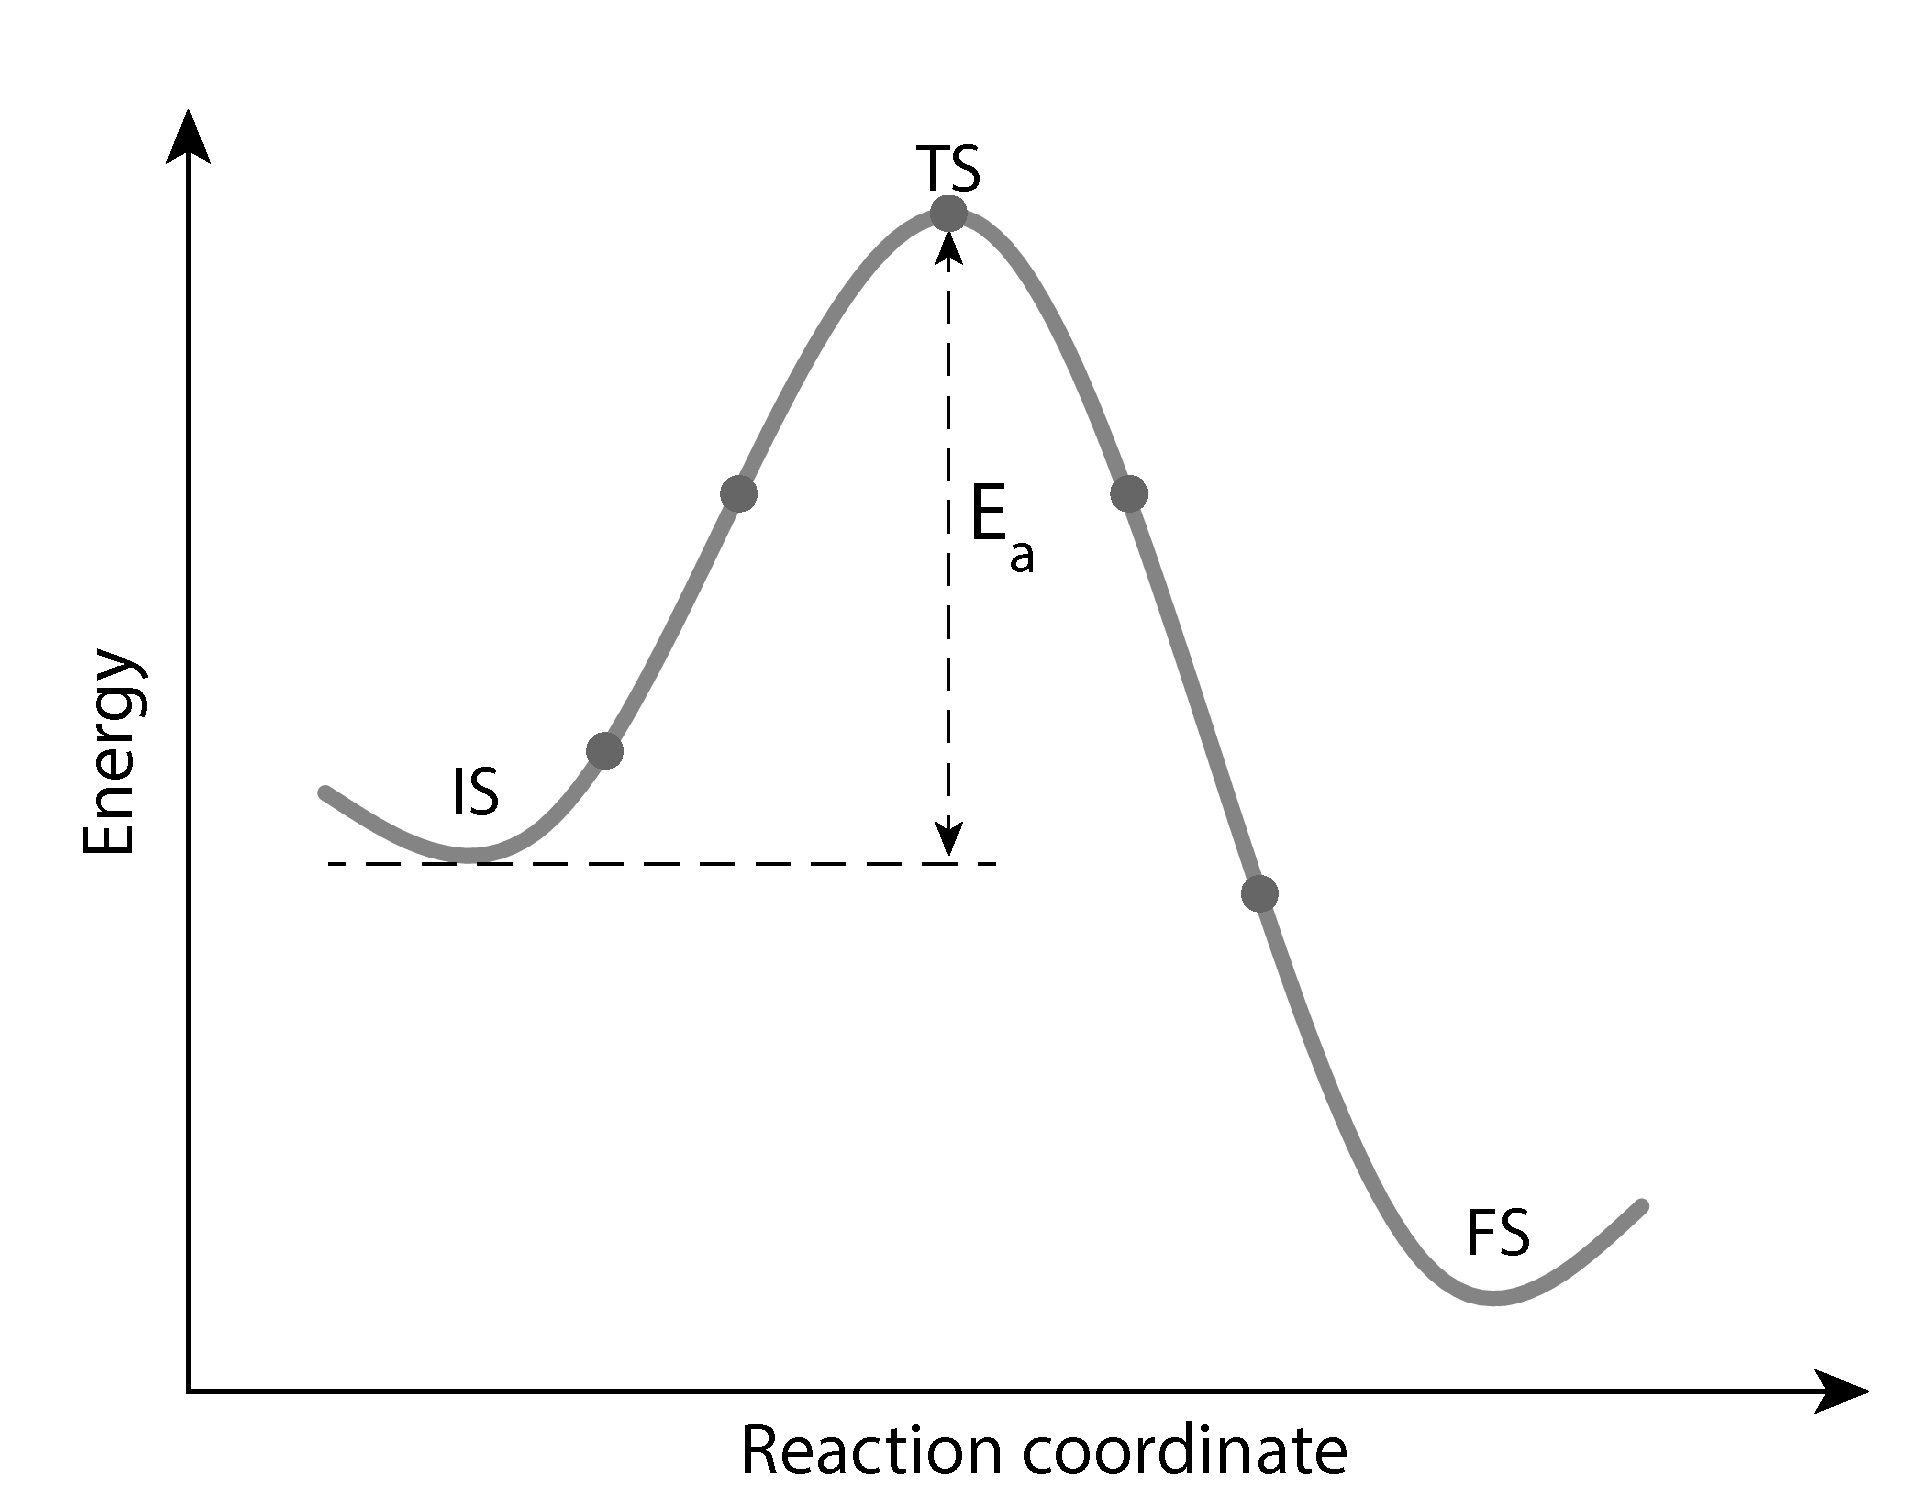
\includegraphics[scale=0.6]{figures/NEB_profile.png}
    \caption{Energy profile of Nudged Elastic Band (NEB) calculation. The IS, TS, and FS are the initial state, transition state and final state, respectively. $E_a$ denotes the activation barrier along the reaction path. The grey circles are the ``images'' in the NEB calculation.}
    \label{fig:NEB_profile}
\end{figure}

The NEB approach initially guesses a number of configurations of several possible intermediate ``images'' that may occur along the reaction coordinate or diffusion path. This set of images can be created by linear interpolation between the initial and final states. The NEB algorithm further conducts constrained optimisation and converges those images along the minimum energy path. Furthermore, fictional spring forces are added between adjacent images to maintain the spacing and the continuity of the reaction or diffusion path. The NEB approach is widely applied in the studies of chemical transformations, such as catalytic reactions or ion diffusion in solid materials. The determined chemical reaction energy barriers can then be used in further, larger time- and length-scale models, such as microkinetic models.\cite{peng2020lithium,Mercer2021}

\subsubsection{Cluster expansion}
\label{sec:cluster_expansion}
The cluster expansion method enables a statistical approach to sample configurational phase space at finite temperature.\cite{sanchez1984generalized,de1994cluster,blum2004mixed} This method aims to capture the energetics of mixing two or more atoms on a given set of lattice sites, typically with an accuracy close to DFT calculations. The approach borrows ideas from the Ising model\cite{gallavotti2013statistical}, where each lattice site is assigned as a spin variable to simulate the magnetic properties, but maps site occupancy onto spin variables instead.\cite{persson2010} For example, for a binary alloy system with atom types A and B, the occupation of each site can be described by a spin-like variable, i.e. $\sigma_i$= +1, if the site is occupied by atom A, and $\sigma_i$= -1 if the site is occupied by atom B, as shown in Figure~\ref{fig:cluster}. A configuration can then be written as $\sigma$=( $\sigma_1$, …, $\sigma_n$). Accordingly, the energy of each configuration can be expressed as: $E\equiv E$($\sigma_1$,…,$\sigma_n$).

\begin{figure}
    \centering
    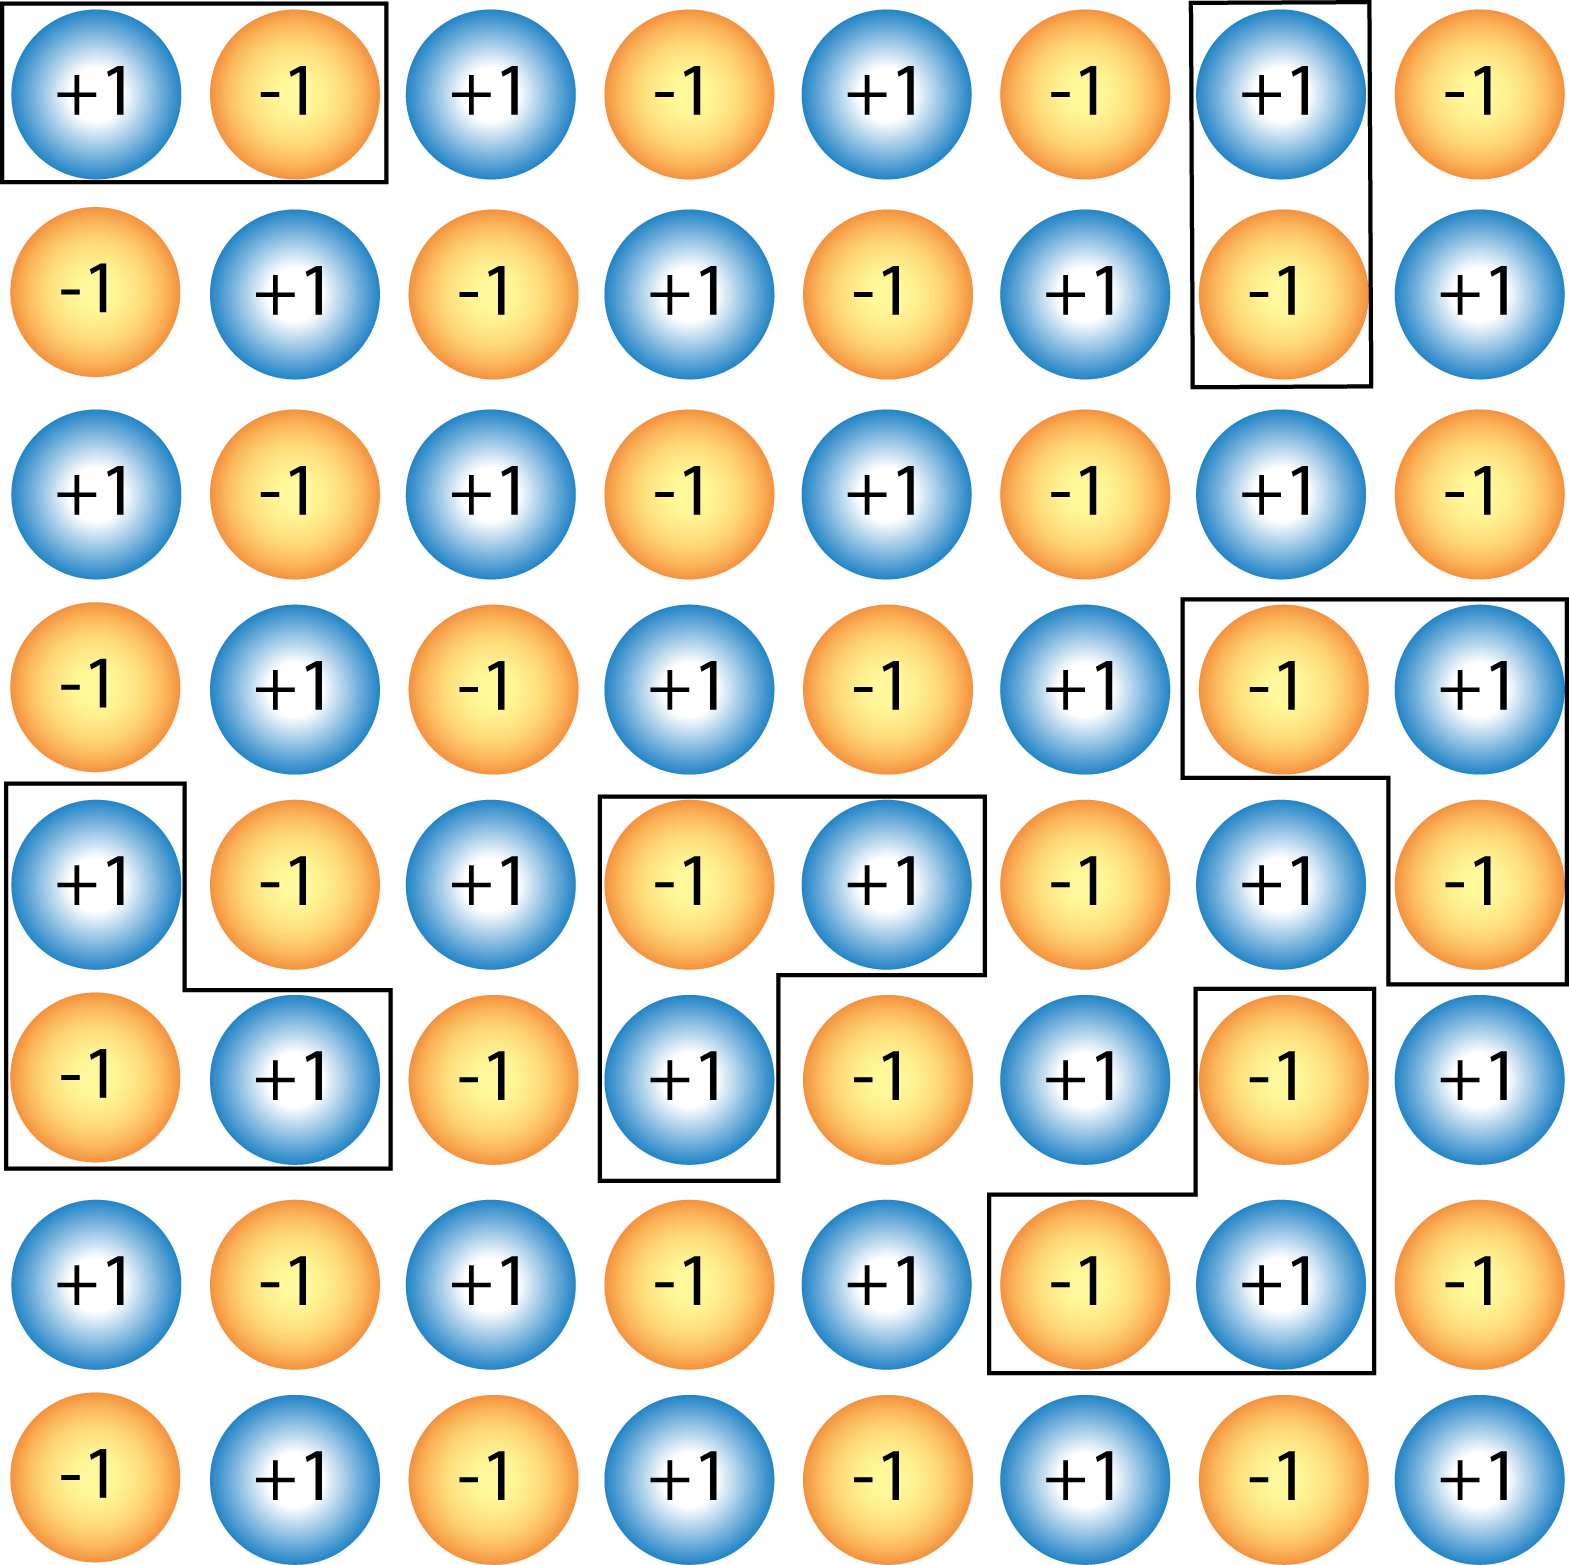
\includegraphics[scale=0.5]{figures/clusters.png}
    \caption{A 2D (8$\times$8) structure including several clusters. +1 and -1 are the lattice sites assigned with different spins.}
    \label{fig:cluster}
\end{figure}

To compute E($\sigma$), all relevant interactions should be sampled. A set of interactions should be considered, such as nearest neighbouring pair interactions, second nearest neighbouring pair interactions, triplet interactions, quadruplet interactions, and so on, up to many body interactions (Figure~\ref{fig:cluster}). Further, all symmetry-equivalent interactions (including translations) can be grouped into ``clusters ($\alpha$)''. Including all relevant cluster interactions, the energy can be expressed as:

\begin{equation}
    \centering
    {E}_{\alpha}=\sum_\alpha {m_\alpha}{J_\alpha}{\bar{\Pi}_\alpha(\sigma)},
    \label{eq:clusters}
\end{equation} 

where $m_\alpha$ is the multiplicity of the cluster, $\alpha$, and can be obtained by considering all the point symmetries in the lattice cell. $J_\alpha$ is the effective cluster interaction (ECI) associated with a cluster, $\alpha$. $\bar{\Pi}_\alpha(\sigma)$ is the correlation matrix of normalised spin-products for a particular cluster of the entire lattice, obtained via:

\begin{equation}
    \centering
    {\bar{\Pi}_\alpha(\sigma)}=\frac{1}{N{m_\alpha}}\sum_{i\in\alpha} {\Pi{\sigma_i}},
    \label{eq:correlation_matrix}
\end{equation} 

where $N$ is the number of parent lattice cells required to generate the configuration $\sigma$. Theoretically, the expansion should include all possible clusters. However, that is not practical and one of the key features of cluster expansions is that they usually converge quickly after including a handful of terms.\cite{VanderVen2001} Consequently, only a relatively small number of \textit{First Principles} calculations are therefore required to parameterise a handful of ECIs. For example, if we calculate the energy of an A-B alloy system and consider only four clusters and four configurations, the energy of each configuration can be expressed as:

\begin{equation}
{\left( \begin{array}{cccc}
{E_1}\\
{E_2}\\
{E_3}\\
{E_4}
\end{array}\right)}=
{\left( \begin{array}{cccc}
{\Pi_1}(1) & {\Pi_2}(1) & {\Pi_3}(1) & {\Pi_4}(1) \\
{\Pi_1}(2) & {\Pi_2}(2) & {\Pi_3}(2) & {\Pi_4}(2)  \\
{\Pi_1}(3) & {\Pi_2}(3) & {\Pi_3}(3) & {\Pi_4}(3)  \\
{\Pi_1}(4) & {\Pi_2}(4) & {\Pi_3}(4) & {\Pi_4}(4) 
\end{array}\right)}
{\left(\begin{array}{cccc}
{J_1}\\
{J_2}\\
{J_3}\\
{J_4}
\end{array}\right)}
\end{equation}

In principle, the effective interaction coefficients, $J_\alpha$, can be obtained via inverting the matrix above and using the energies from \textit{First Principles} calculations, but this is not commonly done. Rather, a larger training set is generated from DFT and the ECIs are fitted in a least-square sense. The set of considered clusters is usually obtained by cross-validation: the set of clusters with the highest accuracy for predicting configurations achieves the highest cross-validation score and is selected.

Various codes exist to link the results of \textit{First Principles} calculations with cluster expansion codes, such as the Alloy Theoretic Automated Toolkit (AT-AT),\cite{avdw:atat2,avdw:atat,VandeWalle2002} the Clusters Approach to Statistical Mechanics (CASM),\cite{natarajan2017} \textit{Ab Initio} Random Structure Search (AIRSS),\cite{Pickard_2011} Integrated Cluster Expansion Toolkit (IceT),\cite{angvist2019} and CLuster Expansion in Atomic Simulation Environment (CLEASE).\cite{chang2019} These codes usually provide a means to fit ECIs and include Monte Carlo (MC) features to sample phase spaces. They also allow the generation of DFT calculations to expand the training set. MC methods are explained in the next section.

\subsubsection{Lattice gas and Monte Carlo}
\label{sec:monte_carlo}

Lattice gas methods simulate the system state as an array of points \cite{Binder2009book}. This data structure is ideally suited to represent periodic, crystalline systems, but extensions to more complex systems are possible. In atomistic simulations, the array values denote the occupation of particular sites by certain types of atoms. The evolution of the system state can then be computed in terms of changes in those array values, i.e. site occupancies.\cite{Binder2009book}
    
In the Ising Hamiltonian described in the previous section, each site can be in either a +1 or -1 state.\cite{lee1952} This data structure is suited to studying the thermodynamics and kinetics of binary alloys.\cite{PMERCER2016394,oviedo2015underpotential} Simplistically, a LiB intercalation material can be represented as a binary alloy of lithium atoms and vacancies within an Ising model.\cite{persson2010,mercer_influence_2017,Kim2001h}   
    
The interaction Hamiltonian describes how the energy of the system depends on the configuration of the lattice. For a simple interaction model, it is possible to perform a direct evaluation of the partition function, $Z$, via:
    
\begin{equation}
        Z = \sum_{i}e^{-\beta E_{i}},
        \label{eq:partition_fn}
\end{equation}

where $E_{i}$ is the energy of state $i$, and $\beta = 1/kT$ ($k =$ Boltzmann constant; $T=$ absolute temperature). Once $Z$ is known, the rest of the thermodynamic properties of the system can easily be determined.\cite{Mercer2019,Leiva2017b,schlueter_quantifying_2018} In a two-level system,\cite{Leiva2017b} the number of states in equation~\ref{eq:partition_fn} can be reduced to scale linearly with the number of particles in the system, making the summation computationally tractable.\cite{Mercer2019,Leiva2017b,schlueter_quantifying_2018} Measurable quantities, like the open circuit voltage (OCV), voltammograms, and partial molar enthalpy and entropy can be simulated.\cite{schlueter_quantifying_2018,Leiva2017b,Mercer2019} This approach has been applied to lithium intercalation in lithium manganese oxide (LMO) \cite{schlueter_quantifying_2018} and graphite,\cite{Mercer2019,Leiva2017b} as demonstrated in section~\ref{sec:anodes_entropy}. The interactions between the particles can be approximated by taking the average occupation in two levels, allowing ordered structures like graphite stages to be modelled. This approach represents a step in complexity beyond the assumption of simple solid solution behaviour, which is still commonly applied in continuum level models. \citeauthor{HAFTBARADARAN2011361} The approach is closely related to the phase field models applied by \citeauthor{Bazant2017} to systems such as lithium iron phosphate (LFP) and graphite \cite{Bazant2017,guo2016,peng2011}.

For a more general and realistic interaction Hamiltonian, the number of energy states precludes direct evaluation of equation~\ref{eq:partition_fn}. In that case, MC methods are useful for calculating thermodynamic properties. This is true for the Ising model defined in section~\ref{sec:cluster_expansion}, when represented in more than one dimension, as is the case in most practical systems.  It is then more practical to obtain the thermodynamic properties by the Metropolis algorithm \cite{Metropolis1953}. Following the Markov chain of states, the limiting distribution equals the probability distribution of the thermodynamic ensemble. Properties of interest can be obtained from taking the average of sampled configurations once the distribution has reached equilibrium \cite{oviedo2015underpotential}.

Inputting a chemical potential, $\mu$, in the grand canonical ensemble, the ground state properties of the system are obtained as follows. For a LiB, $\mu$ represents the chemical potential of intercalated Li in the host, i.e. the electrode potential, described in section~\ref{sec:properties_equilibriumvoltage}. Computing the average occupation, $\langle N \rangle$, of particles in the system at each $\mu$ value, therefore allows the equilibrium potential to be simulated at any input temperature, $T$. Along with $\langle N \rangle$, the average internal energy, $\langle{E}\rangle$, is a useful parameter to check the convergence of the simulation results with respect to the system size \cite{mercer_influence_2017,Binder2009book,Kim2001h,darling1999}.

Variances can be computed to check the system size convergence and derive experimentally measurable parameters. For example, the configurational component of the heat capacity at constant volume, $C_{V}$, given by:

\begin{equation}
    C_{V} = \frac{\beta}{T}\left(\langle{E^{2}}\rangle -{\langle{E}\rangle}^{2}\right) =  \frac{\beta}{T}\rm{var}(E),
    \label{eq:mc_heat_cap}
\end{equation}

where $\rm{var}($E$)$ is the variance of $E$. The vibrational and electronic components of $C_{V}$ must be determined by other means, such as the approaches outlined in section~\ref{sec:thermal_electronic_vibrational}. 

It is also possible to determine voltammograms from $\rm{var}(N)$, as explained by \citeauthor{darling1999} and \citeauthor{mercer_influence_2017}. \cite{darling1999,mercer_influence_2017}. If the covariance of $U$ and $N$ is also known, the partial molar internal energy, $\partial{U}/\partial{N}$ and partial molar entropy $\partial{S}/\partial{N}$ can be obtained, as defined elsewhere \cite{mercer_influence_2017,Kim2001h}. These parameters can be compared with experimental parameters from ``entropy profiling'' or calorimetry \cite{mercer_influence_2017,schlueter_quantifying_2018, Mercer2019,THOMAS2003844,zhang2017} and input into a dynamic model such as kinetic Monte Carlo (kMC) \cite{gavilan-arriazu_kinetic_2020,darling1999,gavilan-arriazu_effect_2020,persson2010}, or Molecular Dynamics (MD) to describe temperature dependent behaviour. A dedicated review of kMC is forthcoming; however, the technique is briefly described by \citeauthor{VanderVen2020}.\cite{VanderVen2020} MD is described in the following section.

\subsubsection{Molecular Dynamics}
\label{sec:molecular_dynamics}
MD is an approach which probes the dynamic evolution of a system over time. The crucial input for these simulations is the potential energy surface (PES), describing the interactions between atoms. In \textit{ab initio} MD (AIMD), this is described by solving the Schr\"{o}dinger equation, whereas in a classical (potentials-based) mechanics framework the interactions are described using parameterised interatomic potentials. Here, we give an overview of both frameworks.

AIMD is able to capture events that potentials-based MD cannot, including bond breaking, and bond formation. AIMD also assumes that the dynamics of particles can be treated classically and that the equation of motion for all particles can be written as:

\begin{equation}
    \label{eq:eom}
    M_I \textrm{\textbf{\"{R}}} _I=-\nabla_I\left[ \varepsilon_0(\textbf{R})+V_{NN}(\mathbf{R})\right],
\end{equation}

where $M_I$ is the mass of a given nucleus, $\textbf{R}$ denotes all nuclear coordinates, $\nabla_I$ is the Laplacian operator of a given nucleus, $\varepsilon_0(\textbf{R})$ represents the ground state energy of the system at that given nuclear configuration, and $V_{NN}(\textbf{R})$ represents the nuclear-nuclear coulomb repulsion at that given nuclear configuration.

Most modern techniques use KS-DFT (c.f. section~\ref{sec:dft}) to solve the Schr\"{o}dinger equation which finds the ground state energy. AIMD can be broadly split up into two main categories: Born-Oppenheimer dynamics and Car-Parrinello extended Lagrangean. The Born-Oppenheimer dynamics method uses a symplectic integrator to numerically integrate the equation of motion in Eq.~\ref{eq:eom} for each time step. The Car-Perrinello extended Lagrangean method gives the Kohn-Sham orbitals an artificial time-dependence. To attain a minimum energy with each new $\textbf{R}$, the orbital dynamics are kept at a temperature much lower than that of the nuclei, but still high enough for the orbitals to quickly relax as the equation of motion proceeds. The new orbitals and their dynamics can then be defined by the Lagrangean equation:\cite{Car1985}

\begin{equation}
    L=\mu \sum_i f_i \int d\textbf{r}|\psi_i(\textbf{r},t)|^2 \
    +\frac{1}{2}\sum^N_{I=1} M_I\dot{\textbf{R}}^2_I (t)- E\left[{\psi(t)}, \textbf{R}(t)\right] \
    +\sum_{i,j} \Lambda_{ij}\left[\int d\textbf{r}\psi^*_{\,i}(\textbf{r},t)\psi_j(\textbf{r}, t)- \delta_{ij}\right],
\end{equation}

where $\mu$ is an artificial kinetic energy term (discussed further in Refs.~\citenum{Tuckerman1994} and \citenum{Grossman2004}), $\psi_x(\textbf{r},t)$ are the time-dependent Kohn-Sham orbitals, and $\Lambda_{ij}$ contains a set of Lagrange multipliers to implement the orthonormality constraint on the orbitals. 

Potentials-based MD is not able to capture some of the finer details of the system dynamics that AIMD is able to, however, it is able to reach longer time- and length- scales, providing information on long range diffusion properties. In classical potentials-based MD, the atomic interactions are described using parameterised interatomic potentials. There are multiple forms interatomic potentials can take, with their relevancy and accuracy relating to the system and study being conducted. Atoms are either attracted or repelled by one another based on their interatomic distance, $r$, to reduce their potential energy to a minimum, $r_{eq}$. This is known as a pair-interaction, which can be used to calculate the force, $\overrightarrow{\rm F}$, acting on each atom, given by:

\begin{equation}
    \overrightarrow{\rm F_i} = \sum_j {\overrightarrow{\nabla}}E(r_{ij})
\end{equation}

In complex systems, there is a ``net effect'' of the $N$ surrounding atoms which can be accounted for by calculating the vector summation of each pair interaction contribution. Within ionic materials, the pair interactions are dominant and therefore it is computationally tractable to truncate the expression after the first term \cite{harding_computer_1990} to give an approximation of the pair potential. The charged nature of ions forms a coulombic interaction, where the relatively slow decay of $\frac{1}{r}$ as $r$ increases, gives rise to the long range component of the potential. The general term for the total potential can therefore be written as:

\begin{equation}
    E(r_{ij}) = \frac{Q_i Q_j}{4\pi \varepsilon_0 r_{ij}} + \Phi_{sr},
\end{equation}

where $i$ and $j$ are ions of charge $Q_i$ and $Q_j$ at a distance of $r_{ij}$, and $\varepsilon_0$ is the permittivity of free space. $\Phi_{sr}$ is used to denote the remaining short-range interactions.

For ionic solids, including cathode materials, a common choice for an interatomic potential is a Coulomb-Buckingham potential \cite{buckingham_classical_1938}, derived from the Born model of the ionic solid \cite{born_1932, mayer_1932}, where the potential energy of the system can be expressed as:

\begin{equation}
    E(r_{ij}) =  \sum_{ij} \frac{Q_i Q_j}{4\pi \varepsilon_0 r_{ij}} + \sum_{ij} A \ exp(\frac{-r_{ij}}{\rho}) - Cr_{ij}^{-6},
    \label{eqn:buckingham}
\end{equation}

where, $A$, $\rho$, and $C$ are constants.

MD simulations can be performed using a range of ensembles, with the most commonly used being microcanonical (NVE), canonical (NVT), and isothermal-isobaric (NPT) ensembles. \cite{todorov2006dl_poly_3, PLIMPTON19951, gale_gulp_1997} Here, the number of atoms (N), volume (V), energy (E), temperature (T), and pressure (P) are conserved within the respective ensembles. Within the NVT and NPT ensembles the energy of endothermic and exothermic processes is exchanged with a thermostat. A variety of thermostat algorithms are available, with some of the most popular methods including the Nos\'{e}-Hoover, Berendsen, and Andersen thermostats. \cite{todorov2006dl_poly_3, PLIMPTON19951, gale_gulp_1997} For NPT ensembles, a barostat is also applied to control pressure.

The choice between AIMD and potentials-based MD is a trade-off between computational cost, accuracy, and transferability. AIMD is highly accurate, however, it is computationally expensive and scales poorly ($>O(N^3)$), making reachable system sizes and timescales relatively small ($<$1000 atoms, $\sim$100 ps). On the other hand, potentials-based MD is less computationally expensive and can be applied to much larger system sizes, up to millions of atoms, with longer reachable time scales in the range of nanoseconds. However, the potentials-based approach is generally less accurate, as developing an interatomic potential which is sufficiently accurate enough to describe the specific system chemistry is challenging. The development of interatomic potentials is discussed in greater detail in section~\ref{sec:potential_fitting}. More recently, development of linear-scaling DFT approaches, as discussed in section~\ref{sec:lsdft}, has worked towards reducing this trade-off.

\subsection{Method Development}

\subsubsection{Continuum models of electrolyte solutions within Density Functional Theory}
\label{sec:dft+cont}
Electrode-electrolyte interfaces are an important part of LiBs and an area of active research.\cite{Gauthier2015, yu2018electrode} The complexity of the structure and formation of electrical double layers at the interface has hindered the understanding of important electrochemical processes. While DFT-based electronic structure methods have been successfully used to study the solid-state physics in the bulk electrodes of LiBs, they are inadequate to describe the liquid state, which lacks structural order. This has led to rapid development of methods to describe the electrode-electrolyte interfaces.\cite{Jinnouchi2018} 

The liquid state can be described mainly via explicit solvation,\cite{Hansen2016} implicit solvation,\cite{Sakong2015} or both.\cite{Skyner2015} In the former, the surrounding solvent and electrolyte molecules are considered at the same level of chemical accuracy as the electrode atoms. The surrounding solvent and electrolyte molecules can not only neutralise the excess charge on the electrode surface, but also form bonds and adsorb on the electrode surface.\cite{Kang2011,Dufils2019, Jorn2013} The addition of a large number of solvent and electrolyte molecules to describe the liquid state drastically increases the configurational degrees of freedom. Sampling this large configurational space is computationally demanding and often leads to loss of focus on the main region of interest: the interface. While consideration of the first bonding layer of explicit solvent and electrolyte molecules is necessary to describe the local effects of bonding and electric field,\cite{Zhang2020} the degrees of freedom of the non-participating solvent and electrolyte molecules far away can be averaged out via an implicit model of the electrolyte solution.\cite{Cramer1999, Tomasi2005} The electrostatic potential in these hybrid quantum-continuum models is obtained from the solution of the Poisson-Boltzmann equation (P-BE).\cite{Grochowski2008} Recently, many DFT codes have integrated P-BE based continuum models.\cite{Jinnouchi2008, Gunceler2013, Ringe2016, Nattino2019, Melander2019, Stein2019, DLMG2018, Dziedzic2020, neutralization-paper}

The continuum electrolyte ions with space-dependent concentrations, $\ci\ofrvec, i=1\dots p$, and charges, $\{z_i\}$, create a mobile electrolyte density, $\rho_{\textrm{mob}}\ofrvec=\sum\limits_{i=1}^p z_i\ci\ofrvec$, which interacts with the quantum charge density, $\rho\ofrvec$, within a mean-field electrostatic potential, $\nu\ofrvec$. This effect can be included in standard DFT by extending the standard free energy functional to include the mean-field electrostatic potential, $\nu\ofrvec$, and the mobile charge concentrations, $\ci\ofrvec$, as:\cite{Dziedzic2020}

\begin{equation}
    E\left[\rho\ofrvec\right]\rightarrow \Omega\left[\rho\ofrvec,\nu\ofrvec,\ci\ofrvec\right]
\end{equation}

The variation of the free energy functional with the electrostatic potential, $\nu\ofrvec$, gives the P-BE:

\begin{equation}
    \label{eq:pbe}
    \nabla\cdot\left[\veps\ofrvec\nabla\nu\ofrvec\right]=-4\pi\left[\rho\ofrvec+\rho_{\textrm{mob}}\ofrvec\right]
\end{equation}

The P-BE not only includes the quantum charge density, $\rho\ofrvec$, as in standard DFT calculations in vacuum, but also the effect of the solvent in terms of a continuum dielectric with permittivity function, $\veps\ofrvec$, and mobile charge density of electrolyte ions, $\rho_{\textrm{mob}}\ofrvec$. The permittivity function is chosen as a smooth function with value varying from 1 in the quantum region to $\veps^\infty$ in the solvent region:\cite{Nattino2019}

\begin{equation}
    \veps\ofrvec=1+\left(\veps^\infty-1\right)s\ofrvec,
\end{equation}

where $s\ofrvec$ is a smooth interface function varying from 0 in the quantum region to 1 in the solvent. Several choices for the interface function have been discussed by \citeauthor{Andreussi2012} \cite{Andreussi2012}. The variation of the free energy functional with ion concentrations, $\ci\ofrvec$, gives the Boltzmann expression for ionic concentrations:

\begin{equation}
    \label{eq:cig}
    \ci\ofrvec = \cif\lambda(\mathbf{r}) \exp \left(-\frac{z_i\nu(\mathbf{r})}{k_{\textrm{B}} T} +\frac{\mu_i^\textrm{ex}}{k_{\textrm{B}} T} \right), \ i=1\dots{}p,
\end{equation}

where $\{\cif\}$ and $\{\mu_i^\textrm{ex}\}$ are the bulk concentrations and excess chemical potentials of the electrolyte ions. The mobile charge density of electrolyte ions, $\rho_{\textrm{mob}}\ofrvec=\sum\limits_{i=1}^p z_i\ci\ofrvec$, is shown schematically in Fig. \ref{fig:DFT+continuum}. As the interaction with mobile electrolyte charge is purely electrostatic and excludes any quantum effects such as Pauli repulsion, there is a problem of electrolyte charge accumulating infinitely close to the electrode. In order to prevent this problem, the models include an electrolyte accessibility function, $\lambda\ofrvec$, which varies from 0 near the electrode to 1 in the bulk electrolyte region.\cite{Fisicaro2017, Sundararaman2018, Stein2019} One of the ways of defining such an accessibility function is as a product of atom-centred interlocking spheres of error functions:\cite{Dziedzic2020}

\begin{figure}
    \centering
    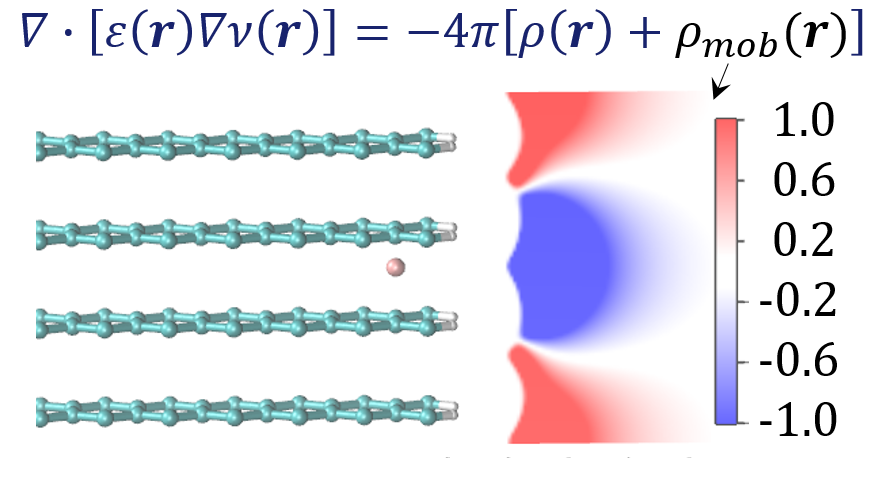
\includegraphics[scale=0.7]{figures/DFT+Continuum.png}
    \caption{DFT simulation of a lithiated graphite interface in contact with an implicit electrolyte solution, based on the solution of the Poisson-Boltzmann equation. Reprinted with permission from Ref.~\citenum{Dziedzic2020}. Copyright 2020 American Chemical Society.}
    \label{fig:DFT+continuum}
\end{figure}

\begin{equation}
    \label{eq:access}
    %\nonumber
    \lambda\ofrvec = \prod\limits_{k}^{n_\textrm{atoms}}\frac{1}{2} \left[1+\textrm{erf}\left(\frac{|\textbf{r}-\textbf{R}_k|-R^{\rm solute}_k(\rho_{\textrm{e}}^\lambda)-R^{\rm solvent}_k}{\sigma}\right)\right],
\end{equation}

where $\sigma$ is a smearing width $(0<\sigma<0.5~a_0)$. This description of the ion exclusion region derives from a physical picture: the electrolyte ions are moved away from the quantum electrode, up to a distance that incorporates not only the size of the species but also a solvation shell radius around the electrolyte ions. The species size can be described in terms of an isoradius of electronic density, $\rho_{\textrm{e}}^\lambda$. The solvation shell radius, $R^{\rm solvent}_k$, depends on the solvent and is added to the species size, to calculate the overall radius of interlocking spheres for the accessibility function.

The electrostatic potential, $\nu\ofrvec$, obtained from equation~\ref{eq:pbe} is due to the entire electrode-electrolyte interface, where the electrode is treated quantum mechanically and the electrolyte solution as a continuum. Variation of the free energy functional with electronic density gives the Kohn-Sham equations in the total electrostatic potential, with additional terms for the variation of interface function with electronic density.\cite{Dziedzic2011, Ringe2016} Solvation energies are defined as:\cite{Ringe2016, Stein2019}

\begin{align}
    \Delta\Omega &=\Omega-\Omega_{\textrm{vac}}-\Omega_{\textrm{electrolyte}} \\
    &=\Omega\left[\rho\ofrvec,\{\ci\ofrvec\},\nu\ofrvec\right] \\
    \nonumber
    &-\Omega\left[\rho_{\textrm{vac}}\ofrvec,\{\ci\ofrvec\}=0,\nu_{\textrm{vac}}\ofrvec\right] \\
    \nonumber
    &-\Omega\left[\rho\ofrvec=0,\{\ci\ofrvec\}=\{\cif\},\nu\ofrvec=0\right]
    \nonumber,
\end{align}

where the respective terms can be computed as the total free energy in the electrolyte solution, the total free energy in vacuum, and the total free energy of the pure electrolyte.\cite{Dziedzic2020} The electrolyte effect on solvation energies can be computed as the difference of solvation energy in electrolyte at $\{\cif\}$ and solvation energy in pure solvent at $\{\cif=0\}$:

\begin{align}
    \Delta\Delta\Omega    &= \Delta\Omega\left[{\{\cif\}}\right]-\Delta\Omega\left[{\{\cif=0\}}\right] \\
    &= \Omega - \Omega_{\textrm{sol}} - \Omega_{\textrm{electrolyte}},
\end{align}

where the respective terms are computed as the total free energy in the electrolyte solution, $\{\cif\}$, the total free energy in pure solvent, $\{\cif=0\}$, and the total free energy of the pure electrolyte. 


\subsubsection{Fitting Potentials for Classical Molecular Dynamics}
\label{sec:potential_fitting}
The development of sufficiently accurate interatomic potentials for a specific chemistry is quite challenging. Interatomic potentials are traditionally based on mathematical functions which has been parameterised using experimental and/or \textit{First Principles} derived data. \cite{jones_1924, buckingham_classical_1938} There are a limited number of codes available with the explicit purpose or functionality for fitting potentials. Here, we present several available codes and discuss the complexities and considerations involved in deriving accurate interatomic potentials.

\textbf{GULP}, \cite{GULP} the General Utility Lattice Program, is a widely used code for performing a variety of simulation types on materials using boundary conditions. \cite{gale_gulp_1997} Within this code, there is the functionality to fit interatomic potentials to either experimental measurements or \textit{First Principles} data.\cite{gale_empirical_1996} GULP is capable of simultaneous fitting to multiple structures and can also handle core-shell models (which capture polarisation of atoms).

\textbf{Atomicrex}, \cite{Stukowski_2017} \textbf{dftfit}, \cite{dftfit} and \textbf{potfit} \cite{wen_kim-compliant_2017, potfit} are codes designed to fit potentials to \textit{First Principles} data. Each of these codes have different levels of flexibility and their own unique features, however, a joint limitation is the ability to fit empirical potentials is limited to rigid ions and cannot fit a core-shell model.

During the process of developing potentials for Li(Ni$_x$Mn$_y$Co$_z$)O$_2$ (NMC), and its ternary system LiNiO$_2$, it was found that none of these codes are able to accurately produce potentials for these materials. The complex nature of Ni chemistry in a layered oxide material is challenging, and to the best of our knowledge, no interatomic potentials exist for Ni$^{3+}$. Oxide systems are widely described using a Buckingham potential form, as given in equation~\ref{eqn:buckingham}, and for layered structures, including NMC and its ternary systems, variations of the Buckingham potentials are presented. Some use rigid ion models,\cite{Lewis_1985, Ledwaba2020, Sayle2005, Dawson0214} others use core-shell models \cite{Hart1998, Fisher2010, Lewis_1985,Ammundsen1999, Kerisit2014, he2019thermal,lee2012atomistic}, and a mixture of formal and partial charges have been implemented. With literature in disagreement over which variation of the Buckingham potential is the most accurate for representing the system, a code capable of fitting different permutations of the Buckingham potential is needed.

Structure and composition of a material are crucial to determine the functional form of the potential. For example, for a layered structure such as NMC-811, it is crucial to consider polarisability. Polarisability is described in classical (potentials-based) MD using a core-shell model. There are predominately two types of core-shell models: the relaxed (massless shells) model \cite{Lindan_1993} and the dynamic (adiabatic shells) model.\cite{Mitchell_1993} The adiabatic shell model is more widely used in literature, including all core-shell related cited works in this section,\cite{Hart1998, Fisher2010, Lewis_1985,Ammundsen1999, Kerisit2014, he2019thermal,lee2012atomistic} for calculating long trajectories, as it is less computationally taxing. In the adiabatic shell model, a fraction of the atomic mass is assigned to the shell. There is no defined fraction size; however, placing 10 \% of the atomic mass on the shell is considered common practice. \cite{PLIMPTON19951,todorov2006dl_poly_3} An additional consideration for using a core-shell model is the separation of the formal atomic charge across the core and shell. However, determined numerical values of the core-shell charge separation are inconsistent.\cite{wang2014molecular,escribano2017enhancing, lee2012atomistic,Lee2013_lithium,dai2019comparison} In some systems, where there is high polarisability, such as in LMO, the short-range interactions are overwhelmed by the longer-range coulombic term. In these cases, the system charges can be scaled to increase the influence of the short-range interactions, and are termed partial charges. The scaling factor is system dependent therefore no specific value is ideal in all cases, however 60 \% formal charge is commonly adopted. \cite{pedone2006potentials}

POtential Parameter Optimisation for Force-Fields (PopOff),\cite{Morgan2021PopOff} a code developed within the Faraday institution, was specifically created for fitting different permutations of the Buckingham potential. It is unique in its ability to consider all the factors discussed above (rigid ion/core-shell/charge separation/charge scaling) in a modular design, allowing flexible fitting to suit individual systems. The code has been developed in Python, using a training set consisting of DFT derived data ($DFT$) and utilising the Large-scale Atomic/Molecular Massively Parallel Simulator (LAMMPS).\cite{PLIMPTON19951} The potential is fitted by minimising the mean squared error ($\chi^2$) between the DFT forces, $F^{DFT}$, and stress tensors, $\sigma^{DFT}$, and those produced using the fitted interatomic potential ($F^{IP}$, $\sigma^{IP}$), defined as:

\begin{equation}
    \chi^2 = \sum^{N}_{i,\alpha} \frac{(F^{DFT}_{i,\alpha} - F^{IP}_{i,\alpha})^2}{N_i} +  \sum_{\beta} \frac{(\sigma^{DFT}_{\beta} - \sigma^{IP}_{\beta})^2}{6}
\end{equation}

This modular design allows the construction of a Buckingham potential able to accommodate the considerations and complexities of different systems. PopOff also allows for individual parameters to be fixed/excluded from the fit, lowering the fit dimensionality and computational cost. This is particularly useful for excluding dispersion terms, which are known to be zero or close to, for a range of elements.\cite{Lee2013_lithium,fisher2008lithium}

\subsection{Calculating observable properties}
\subsubsection{Equilibrium voltage}
\label{sec:properties_equilibriumvoltage}
The equilibrium cell voltage, $E(x)$, where $0 < x < 1$ denotes the fraction of sites occupied by lithium in the intercalation host, is a fundamental thermodynamic quantity related to the energy density of a cell \cite{Urban2016,CEDER1999131,VanderVen2020}. $E(x)$ can be probed through experimental measurements of the open circuit voltage (OCV), that is, the voltage between the cathode and anode terminals under zero current flow, assuming that the system has been given sufficient time for the OCV to relax to the value of $E(x)$. Computationally, the equilibrium cell voltage can be modelled through \textit{First Principles} calculations at $T = 0$ K \cite{Urban2016,CEDER1999131,VanderVen2020}; the effect of thermal fluctuations can be included by modelling using Monte Carlo (MC) calculations \cite{mercer_influence_2017,Kim2001h}.

There is a fundamental relationship between the Gibbs free energy of lithium dissolution into the host, $G(x)$, the chemical potential of Li intercalation in the host, $\mu(x)$, and the cell voltage $E(x)$. Knowledge of $G(x)$ also provides information about the evolution of the phase behaviour dependent on the fraction of intercalated Li,\cite{CEDER1999131,persson2010,VanderVen2020,VanDerVen2000b} enabling the construction of phase diagrams from \textit{First Principles}. The relationships are represented schematically in Figure~\ref{fig:vanderven_thermodynamics}. In essence: the tangent to the free energy curve, $G(x)$, allows $\mu(x)$ and hence the cell voltage to be obtained. Alternatively, integration of $\mu(x)$ can be used to derive free energy curves.

\begin{figure}
    \centering
    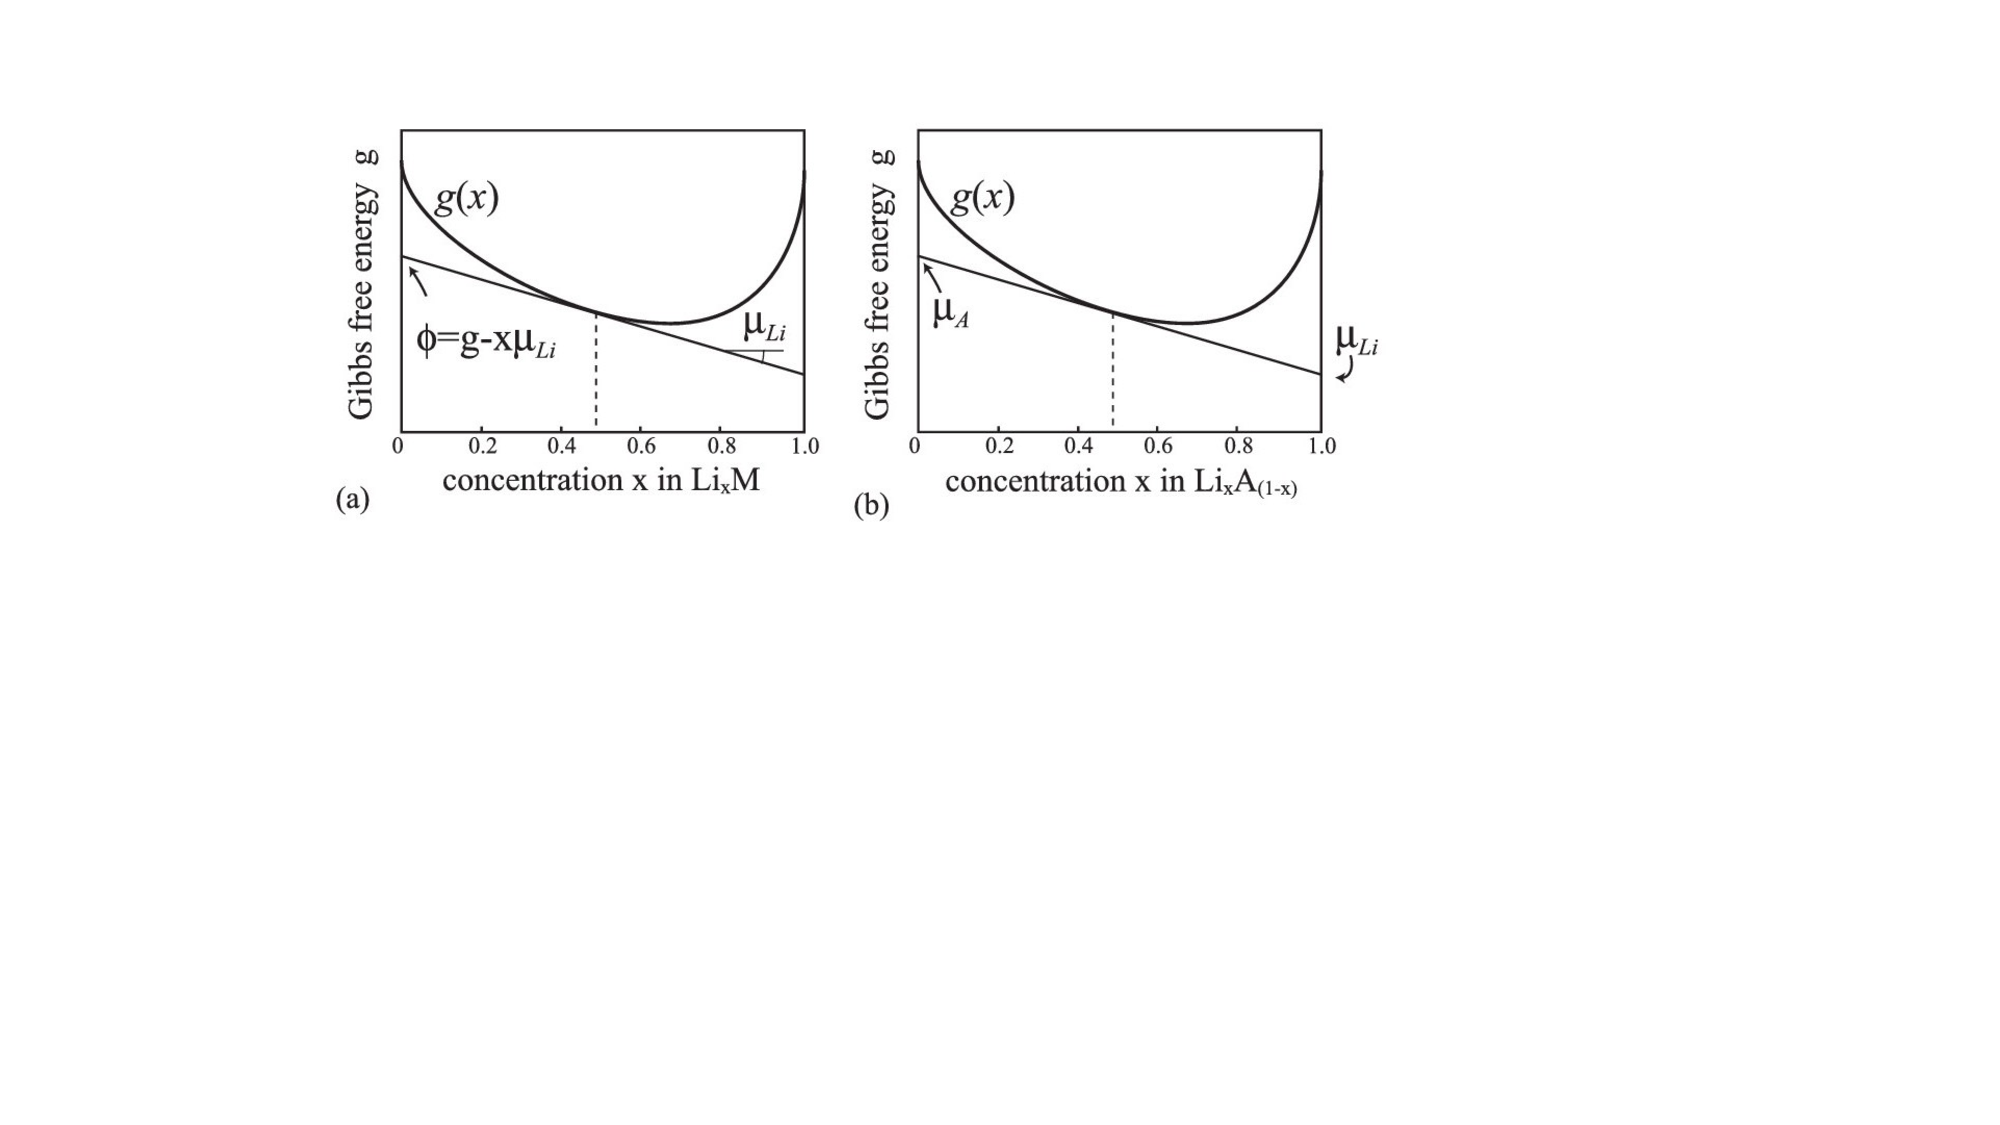
\includegraphics[scale=0.8]{figures/thermodynamics_vanderven.pdf}
    \caption{Representation of the connection between the Gibbs free energy, $G(x)$, the  lithium chemical potential $\mu(x)$ in (a) an intercalation electrode and (b) an alloy electrode. Reprinted with permission from Ref.~\citenum{VanderVen2020}. Copyright 2020 American Chemical Society.}
    \label{fig:vanderven_thermodynamics}
\end{figure}

In the case of a Li-ion cell, the equilibrium cell voltage, $\phi(x)$, and the chemical potential of intercalated Li, $\mu(x)$, are related by:

\begin{equation}
    \phi(x) = -\frac{\mu(x) - \mu_{\rm{Li}}^{\rm{ref}}}{nF},
    \label{eq:potchempot_raw}
\end{equation}

where $\mu_{\rm{Li}}^{\rm{ref}}$ is the chemical potential of the reference electrode, $n$ is the number of electrons transferred per formula unit of intercalation host ($n =1$ for Li-ion cells), and $F$ is the Faraday constant. The most convenient reference potential, both from the point of view of simulations and for comparison with experimental measurements of Li-ion half cells, is the bcc metallic Li anode. With a suitable choice of units for all potentials ($\mu$ expressed in eV per formula unit of intercalation host), equation~\ref{eq:potchempot_raw} can be written much more simply as:\cite{CEDER1999131}

\begin{equation}
    \phi(x) = -\mu(x)
    \label{eq:potchempot}
\end{equation}

The intercalated Li chemical potential is defined by:

\begin{equation}
    \mu(x) = \left(\frac{\partial{\underline{G}(x)}}{\partial{N_{Li}}}\right)_{p,T,N_{\rm{host}}} = \left(\frac{\partial{G(x)}}{\partial{x}}\right)_{p,T,N_{\rm{host}}},
    \label{eq:chemicalpotgibbs}
\end{equation}

where $\underline{G}$ is the absolute (i.e. extensive) Gibbs free energy of Li dissolution into the host, $p$ is pressure, $T$ is the absolute temperature, and $N_{\rm{host}}$ and $N_{\rm{Li}}$ are the number of host and lithium atoms in the system, respectively. The subscripts $p$, $T$, and $N_{\rm{host}}$ will be implicitly assumed to be constant from now on and dropped, to simplify notation.

Similarly, it is well known that:

\begin{equation}
    \frac{\partial{G(x)}}{\partial{x}} = \frac{\partial{H(x)}}{\partial{x}} - T\frac{\partial{S(x)}}{\partial{x}}, 
    \label{eq:gibbshs}
\end{equation}

where $H(x)$ and $S(x)$ are the enthalpy and entropy, respectively, per formula unit of host material.

We can use equations \ref{eq:potchempot}, \ref{eq:chemicalpotgibbs}, and \ref{eq:gibbshs} to get $\partial{G}/\partial{x} = -E_{\rm{OCV}}$, then, taking the derivative of the OCV with respect to $T$ and using the chain rule, we obtain:

\begin{equation}
   \frac{\partial{S(x)}}{\partial{x}} = \frac{\partial{E_{\rm{OCV}}(x)}}{\partial{T}}
    \label{eq:entropy_measurement}
\end{equation}

and so:

\begin{equation}
    \frac{\partial{H(x)}}{\partial{x}} = T\frac{\partial{E_{\rm{OCV}}(x)}}{\partial{T}} - E_{\rm{OCV}}(x)
    \label{eq:enthalpy_measurement}
\end{equation}

Due to the units of electron Volts (eV) per formula unit for the potentials $H(x)$ and $TS(x)$, i.e. as in the conversion between equations~\ref{eq:potchempot_raw} and \ref{eq:potchempot}, the usual factors of $F$ have been omitted. In this way it is possible to simulate not only the equilibrium voltage, but split its contributions into enthalpy and entropy components. Both components can be experimentally measured \cite{schlueter_quantifying_2018, Mercer2019, THOMAS2003844,Reynier2004,Yazami_2006} and modelled through MC or mean field methods \cite{schlueter_quantifying_2018,mercer_influence_2017,Mercer2019,Leiva2017b}, providing additional properties for model validation purposes and to check the temperature dependence of those properties is modelled accurately. A good thermodynamic basis can then be used to derive dynamic properties, as outlined in the subsequent sections.

\subsubsection{Activity coefficients of electrolytes}
\label{sec:tf}
The activity coefficients of electrolytes ($\gamma_j$, $j=1\dots p$) describe the thermodynamics of non-ideal solutions.\cite{Atkins2014} The activity coefficient of electrolytes can be computed from DFT+P-BE models, as described in section~\ref{sec:dft+cont}, by computing the electrolyte effect on solvation energies, $\Delta\Delta\Omega$:\cite{Ringe2016, Dziedzic2020}

\begin{equation}
    \label{eq:activityj}
   \ln{\gamma_j}  =\frac{\Delta\Delta\Omega_j\left[\{\cif\}\right]}{k_{\textrm{B}} T}, \ j=1\dots p
\end{equation}

For an electrolyte dissociating into $p$ species, the mean activity coefficient can be calculated as:

\begin{equation}
    \label{eq:activitymean}
    \ln \gamma_{\rm mean} = \frac{1}{p}\sum_{j=1}^p \ln \gamma_j
\end{equation}

\subsubsection{Diffusion coefficients}
\label{sec:diffusion}
The \textit{diffusion coefficient} is a term used to describe the rate of ion transport within a system. This term, however, has been used in literature to express several forms of diffusion, which characterise diffusion in a material in different ways. Here, we describe several commonly used forms of \textit{diffusion coefficient}, in context of where they are used, focusing on bulk diffusion. \citeauthor{heitjans2006diffusion} gives a detailed description of diffusion along grain boundaries and along surfaces (chapters 7 and 8).\cite{heitjans2006diffusion}

Ionic transport within the electrodes and electrolyte plays a vital role in the kinetics of a battery. It can be described fundamentally with flux expressions that relate ion fluxes to chemical or electrochemical potential gradients. This is related by Fick's first law, where the diffusion flux, $\boldsymbol{\jmath}$, is described using the gradient of the concentration, $c$, via:

\begin{equation}
    \boldsymbol{\jmath} = - \mathcal{D} \nabla c,
    \label{eq:fickfirst}
\end{equation}

where $\mathcal{D}$ is denoted as the diffusion coefficient tensor or diffusivity tensor and implies that $\mathcal{D}$ varies with direction. In general, the diffusion flux and concentration gradient are not always antiparallel. They are antiparallel for isotropic mediums. \citeauthor{heitjans2006diffusion} discusses this in more detail.\cite{heitjans2006diffusion}

Steady state methods for measuring diffusion coefficients, like the permeation method, are directly based on Fick's first law.\cite{heumann2013diffusion} In non-steady states, the diffusion flux and concentration vary with time, $t$, and position $x$, and a balanced equation is necessary. For particles which undergo no reaction this become the continuity equation:

\begin{equation}
    \frac{\partial c}{\partial t} + \nabla {\boldsymbol{\jmath}} = 0
    \label{eq:continuity}
\end{equation}

Combining equations \ref{eq:fickfirst} and \ref{eq:continuity} leads to Fick's second law, also called the diffusion equation, which predicts how diffusion causes the concentration to change with time:

\begin{equation}
    \label{eq:ficksecond}
    \frac{\partial c}{\partial t} = \nabla (\mathcal{D} \nabla c )
\end{equation}

In diffusion studies with trace elements the material composition does not practically change and $\mathcal{D}$ is independent of the tracer concentration, presenting a concentration-independent diffusion coefficient. For diffusion in multiple dimensions Fick's second law becomes: \cite{crank1979mathematics}

\begin{equation}
    \frac{\partial c}{\partial t} = \mathcal{D} \nabla^2 c
    \label{eq:nodirectional_diffusion}
\end{equation}

The temperature dependence of the diffusion coefficient is often described empirically by an Arrhenius relation:

\begin{equation}
    \mathcal{D} = \mathcal{D}_0 \cdot \textrm{exp} \left (- \frac{E_A}{k_B T} \right ),
\end{equation}

where $E_A$ is the activation energy for the mass transport, $D_0^T$ is the pre-exponential factor, $k_B$ is the Boltzmann constant, and $T$ is the temperature.

From the microscopic point of view, the tracer diffusion coefficient can be defined by the Einstein-Smoluchowski relation: \cite{einstein1905presumed,von1906kinetischen}

\begin{equation}
    \mathcal{D} = \lim_{t\to\infty} \frac{\left <r^2(t)\right >}{2dt}, \mathrm{where} \left <r^2(t)\right > = \left< \left(x(t) - x_0 \right)^2 \right>,
    \label{eq:self-diffision}
\end{equation}

where, $\left <r^2(t)\right >$ is the mean square displacement (MSD) of the particles after time $t$ and $d$ is the dimensionality of the movement. This is also known as the \textit{self diffusion coefficient} and is the main approach used to calculate the diffusion coefficient in kMC and MD from the atom trajectories. \citeauthor{VanderVen2020} discusses in greater detail.\cite{VanderVen2020}

In atomistic modelling, diffusion coefficients can also be calculated using other approaches, such as Green-Kubo. The Green-Kubo approach is linked to the Einstein-Smoluchowski relation approach, equation~\ref{eq:self-diffision}. Both approaches assume that particle dynamics can be well approximated by Brownian motion. As described in equation~\ref{eq:self-diffision}, Brownian motion of independent particles can be expressed by the MSD of a particle proportional to time. This can also be termed as the integral of the velocity. The Green-Kubo approach is derived from the integration of the velocity (or current) autocorrelation function. Assuming that dynamics is ergodic, the diffusion coefficient can be calculated using a linear fit to the velocity autocorrelation function. Averaging is applied to this, for example, a time  average for a selected particle type, a sample average, or an ensemble average.


\subsubsection{Vibrational and Thermal Properties}
\label{sec:thermal_electronic_vibrational}
While MD simulates the evolution of a chemical system over time, lattice dynamics is an approach that models the underlying vibrations. In crystalline solids, extended vibrations can be described as phonons with a characteristic frequency and wavevector, $\omega(q)$. A unit cell with $N$ atoms contains 3$N$ phonon modes. The theory of phonons provides a direct connection between microscopic atomic motion and macroscopic properties including specific heat capacity, IR and Raman spectra, and thermal expansion.\cite{ladd1986lattice, turney2009predicting,seko2015prediction} 

While assuming that phonons are harmonic simplifies the theoretical description, it is necessary to include anharmonic effects to describe phenomena such as heat transport. The lattice thermal conductivity, $\kappa$, depends on the lifetime of each phonon, i.e. how long it persists before decaying, which is an anharmonic process. Formally, the thermal conductivity given by the product of the modal heat capacity, ($C_V$), the group velocity, $v$, and the phonon mean free path, $v \times \tau$ (where $\tau$ is the phonon lifetime). The macroscopic $\kappa$ is obtained by summing over band indices, $v$, averaging over wavevectors, $q$, and normalising by the unit cell volume:

\begin{equation}
    \kappa = \frac{1}{NV_0} \,\sum_{qv} C_{V,qv} v_{qv} \otimes v_{qv} \tau_{qv},
    \label{eq:thermal}
\end{equation}

where $N$ is the number of unit cells in the crystal (number of wavevectors in the Brillouin zone summation) and $V_0$ is the volume of the crystallographic unit cell.

The heat capacity and group velocity can be extracted from the harmonic phonons, which are readily accessible from calculations based on \textit{First Principles} or potentials-based potential methods. The lifetime of each phonon mode is more demanding to compute and is often performed within a many-body perturbation theory expansion of phonon-phonon interactions. One approximation is to consider only the leading term of three-phonon creation and annihilation. \cite{togo_distributions_2015} However, higher-order processes may limit the lifetimes, depending on the material and temperature. There are a range of packages available to compute the terms in equation~\ref{eq:thermal} including \textsc{Phono3py} \cite{togo_distributions_2015} (recently applied to \ce{LiCoO2} and NMC cathodes)\cite{yang2019highly,yang2020chemical}, \textsc{ALAMODE}\cite{tadano2014anharmonic}, and \textsc{ShengBTE}\cite{ShengBTE_2014}.

 \end{document}